\documentclass[a4paper,11pt,twoside]{article}

\usepackage{my-thesis-template}


%----------------------------------------------------------------------------------------
%	METADATA
%----------------------------------------------------------------------------------------
\newcommand{\thesistitle}{Robotic surgical tool manipulator - Recognition, control and manipulation of laparoscopic tools}
\newcommand{\division}{Division}
\newcommand{\me}{Karadimos Alexios of Loukas}
\newcommand{\nomme}{Karadimos Alexios of Loukas}
\newcommand{\studnum}{1046820}
\newcommand{\monthyear}{Month 2021}
\newcommand{\supname}{Evangelos Dermatas}
\newcommand{\suptitle}{Associate Professor Dr.}
\newcommand{\cosupname}{Anthony Tzes}
\newcommand{\cosuptitle}{Professor Dr.}
\newcommand{\headofdivision}{Kazakos Demosthenes}
\newcommand{\headofdivisiontitle}{Assistant Professor Dr.}
\newcommand{\keywords}{surgery, robotics, control, laparoscopy}
\title{\thesistitle}
\author{Karadimos Alexios}
\date{2020}

% PDF metadata
\hypersetup
{
    pdfauthor={Alexios Karadimos},
    pdftitle={thesis},
    pdfsubject={\thesistitle},
    pdfkeywords={\keywords},
    pdfproducer={PdfLaTex},
    pdfcreator={Alexios Karadimos}
}


\begin{document}

\selectlanguage{greek}
\selectlanguage{english}


%----------------------------------------------------------------------------------------
%	FRONT PAGE & CERTIFICATION
%----------------------------------------------------------------------------------------
\begin{titlepage}
\begin{center}
% Upper part of the page
\textsc{\textbf{\large UNIVERSITY OF PATRAS - SCHOOL OF ENGINEERING}\\
\large DEPARTMENT OF ELECTRICAL AND COMPUTER ENGINEERING}\\

\includegraphics[width= 0.5\textwidth]{up_2017_logo_gr.png}\\  

\textsc{Division: \large Systems and Automatic Control}\\[1cm]

\textsc{\textbf{\LARGE{Thesis}}}\\ [0.5cm]
of the student of the Department of Electrical and Computer Engineering of the School of Engineering of the University of Patras\\[0.5cm]

\textsc{\Large \me }\\[0.5cm]
\textsc{\large Student Number: 1046820}\\[1cm]

\underline{\large Subject}\\
\HRule \\[0.4cm]
{\huge \bfseries \thesistitle }\\[0.4cm] % Title of your document
\HRule \\[1.5cm]

\underline{\large Supervisor}\\[0.5cm]
\large \suptitle \, \supname \\[1cm]
\textbf{Thesis Number:}
%\large 1046820/2020
\vfill
% Bottom of the page
\large{Patras, 2020}
\end{center}
\end{titlepage}

% \begin{titlepage}

% %----------------------------------------------------------------------------------------
% %	HEADING SECTIONS
% %----------------------------------------------------------------------------------------

% \Large UNIVERSITY OF PATRAS - SCHOOL OF ENGINEERING\\[0.5cm] % Name of your university/college
% \textsc{\Large DEPARTMENT OF ELECTRICAL AND COMPUTER ENGINEERING}\\[0.5cm] % Major heading such as course name
% \textsc{\large \textlatin{ECE}ΔΚ803}\\[0.5cm] % Minor heading such as course title

% %----------------------------------------------------------------------------------------
% %	TITLE SECTION
% %----------------------------------------------------------------------------------------


% %----------------------------------------------------------------------------------------
% %	AUTHOR SECTION
% %----------------------------------------------------------------------------------------


% % If you don't want a supervisor, uncomment the two lines below and remove the section above
% %\Large \emph{Author:}\\
% \emph{Αλέξιος Καραδήμος}\\ % Your name
% Τμήμα Ηλεκτρολόγων Μηχανικών \& Τεχνολογίας Υπολογιστών\\[2cm]

% %----------------------------------------------------------------------------------------
% %	DATE SECTION
% %----------------------------------------------------------------------------------------

% {\large 2020}\\[1cm] % Date, change the \today to a set date if you want to be precise

% %----------------------------------------------------------------------------------------
% %	LOGO SECTION
% %----------------------------------------------------------------------------------------

% \begin{center}
% \includegraphics[width=5cm]{images/up_2017_logo_gr.png}\\[1cm] % Include a department/university logo - this will require the graphicx package
% \end{center}

% %----------------------------------------------------------------------------------------

% \vfill % Fill the rest of the page with whitespace

% \end{titlepage}

\pagestyle{empty}
\begin{center}
{\LARGE \textbf{CERTIFICATION}\\[1cm]}
\large It is certified that the Diploma Thesis titled\\[1cm]
\textbf{\large \thesistitle }\\[1cm]
of the Department of Electrical and Computer Engineering student\\[1.5cm]
\textbf{\large \me }\\[0.5cm]
Registration Number: \studnum \\[1.5cm]
was presented publicly at the Department of Electrical and Computer Engineering at\\[0.5cm]
\Large{02/02/2022}\\[0.5cm]
and was examined by the following examining committee:\\[0.5cm]
\supname, \suptitle (supervisor)\\
Konstantinos Moustakas, Professor (committee member)\\
Kyriakos Sgarbas, Associate Professor (committee member)\\
\end{center}

\vfill

\begin{minipage}{0.5\textwidth}
\begin{flushleft} \large
The supervisor\\[3cm]
\supname \\
\emph{\suptitle}
\end{flushleft}
\end{minipage}
\begin{minipage}{0.5\textwidth}
\begin{flushright} \large
The Director of the Division\\[3cm]
\headofdivision\\
\emph{\headofdivisiontitle}
\end{flushright}
\end{minipage}

\pagestyle{empty}
\begin{center}

{\large \textbf{Thesis details}\\[1cm]}

\textbf{\large \thesistitle }\\[1cm]

\pagestyle{empty}
{\textbf{Abstract}\\[1cm]}

This thesis studies all the stages involved in the recognition, control and manipulation of laparoscopic tools in an end-to-end approach with more emphasis given to the pivot trajectories and the RCM constrained motion 
planning. The first step was to study the forward and inverse kinematics of the KUKA iiwa14 industrial robot arm (with the position-orientation decoupling technique for 6dof robots, leaving the extra degree of freedom to be 
specified by other constraints) as well as kinematics of the Barrett hand gripper in order to calculate grasps. Since MIS robotics is very constrained in nature, the next step was to study the RCM constraint for the pivot 
motions, the elbow-up constraint to avoid collisions as well as the workspace constraints and singularities. When designing robot applications it is important to study the robot’s workspace, and for this reason, this thesis 
also studies the surgical task space and how this is transformed to the robot’s taskspace and the joint space. The manipulability of the robot was also studied and also a suitable environment layout so that all trajectories 
were well reachable. A lot of emphasis was given in calculating various geometric paths for the robot to follow inside the surgical task. The equations for circular, circular arc, line segment, helical, cubic spline, b-spline, 
higher-order polynomial and trapezoid and s-curve velocity profile trajectories are studied in detail in order to generate pivot motions with a wide variety. All experiments were conducted using the ROS framework and popular 
tools and libraries like Gazebo, RViz and MoveIt using the RRTConnect path planning algorithm. The experiments were evaluated with measurements of time, position accuracy and RCM distance deviation. This thesis also briefly 
studies a simple recognition of a laparoscopic tool and the estimation of it’s position and orientation using computer vision as well as the calculation of 3 points on the surgical tool where the gripper’s fingers will be 
placed in order to grasp the object with a satisfactory force closure. Finally this thesis studies some control system schemes like for example the RCM tracking and pivot motion control.

\newpage{\pagestyle{empty}\cleardoublepage}

\newpage
\pagestyle{empty}
{\textbf{Περίληψη}\\[1cm]}

Η παρούσα διπλωματική εξετάζει όλα τα στάδια που εμπλέκονται στην αναγνώριση, τον έλεγχο και τον χειρισμό των λαπαροσκοπικών εργαλείων με μια ολιστική προσέγγιση αλλά με μεγαλύτερη έμφαση να δίνεται στις τροχιές περιστροφής 
γύρω από σημείο και στον προγραμματισμό περιορισμένης κίνησης RCM. Το πρώτο βήμα ήταν να μελετηθεί το ευθύ και αντίστροφο κινηματικό πρόβλημα του βιομηχανικού ρομποτικού βραχίονα KUKA iiwa14 (με την τεχνική αποσύνδεσης θέσης-
προσανατολισμού για ρομπότ 6 βαθμών ελευθερίας, αφήνοντας τον επιπλέον βαθμό ελευθερίας να καθοριστεί από άλλους περιορισμούς) καθώς και η κινηματική της αρπάγης Barrett ώστε να υπολογιστούν λαβές του χειρουργικού εργαλείου. 
Δεδομένου ότι η ρομποτική MIS επιβάλλει πολλούς περιορισμούς, το επόμενο βήμα ήταν να μελετηθεί ο περιορισμός RCM για τις κινήσεις περιστροφής (pivot), o περιορισμός στον οποίο ο αγκώνας του ρομπότ πρέπει να είναι προς τα πάνω 
για την αποφυγή συγκρούσεων καθώς και οι περιορισμοί και τα σημεία ενικότητας του χώρου εργασίας. Κατά το σχεδιασμό εφαρμογών ρομπότ είναι σημαντικό να μελετηθεί ο χώρος εργασίας του ρομπότ και για το λόγο αυτό, αυτή στη 
διπλωματική αυτή μελετάται επιπλέον ο χώρος χειρουργικών εργασιών και πώς αυτός μετατρέπεται στον χώρο εργασιών του ρομπότ και στον χώρο αρθρώσεών του. Μελετήθηκε επίσης ο δείκτης επιδεξιότητας του ρομπότ και η κατάλληλη 
διάταξη του ρομπότ σε σχεση με το περιβάλλον του έτσι ώστε όλες οι τροχιές να είναι καλά προσβάσιμες και να μπορουν να εκτελεστούν με ευκολία. Δόθηκε μεγάλη έμφαση στον υπολογισμό διαφόρων γεωμετρικών μονοπατιών που έπρεπε να 
ακολουθήσει το ρομπότ μέσα στο χώρο χειρουργικής εργασίας. Οι εξισώσεις για τροχιές κύκλου, κυκλικού τόξου, ευθύγραμμου τμήματος, έλικα, κυβικού spline, b-spline, πολυωνύμων υψηλότερης τάξης και τροχιές με προφίλ ταχύτητας 
τραπεζοειδές και καμπύλης-s, μελετώνται λεπτομερώς, προκειμένου να δημιουργηθούν χειρουργικές ρομποτικές κινήσεις με μεγάλη ποικιλία. Όλα τα πειράματα υλοποιήθηκαν χρησιμοποιώντας το περιβάλλον ROS και δημοφιλή εργαλεία και 
βιβλιοθήκες όπως τα Gazebo, RViz και MoveIt χρησιμοποιώντας τον αλγόριθμο σχεδιασμού διαδρομής RRTConnect. Τα πειράματα αξιολογήθηκαν με μετρήσεις χρόνου, ακρίβειας θέσης και απόκλισης απόστασης RCM. Στη διπλωματική αυτή 
μελετάται επίσης εν συντομία η απλή αναγνώριση ενός λαπαροσκοπικού εργαλείου και η εκτίμηση της θέσης και του προσανατολισμού του με χρήση υπολογιστικής όρασης καθώς και ο υπολογισμός 3 σημείων πάνω στο χειρουργικό εργαλείο 
όπου θα τοποθετηθούν τα δάχτυλα της αρπάγης για να πιάσει το αντικείμενο με μία ικανοποιητική λαβή. Τέλος, σε αυτή τη διπλωματική μελετώνται ορισμένα συστήματα ελέγχου όπως για παράδειγμα ενός συστήματος για την παρακολούθηση 
RCM και τον έλεγχο κίνησης περιστροφής.


\pagestyle{empty}
{\textbf{Αcknowledgements}\\[1cm]}

The subject of this thesis, is a subject that I have been passionate about for many years and from the beginning of my university studies. For this reason 
I would like to thank my supervisors for giving me the opportunity to dive deep into this fascinating subject. I would also like to thank my friends and 
family for their huge support and for pushing me during the pandemic to conquer my academic goals.



%----------------------------------------------------------------------------------------
%	TABLE OF CONTENTS
%----------------------------------------------------------------------------------------

\pagestyle{fancy}

\clearpage
\tableofcontents
\renewcommand*\contentsname{Table of Contents}

%----------------------------------------------------------------------------------------
%	MAIN SECTIONS
%----------------------------------------------------------------------------------------

\newpage
\chapter{Introduction}

\section{Surgical robotics}

\subsection{Historical Overview of Surgical robotics}

Surgical robotics is a field of Surgery where the surgeon operaties on the patient via a computer, specialised equipment and robotic arms, 
to which the surgical tools needed for the operation are attached. According to surgical bibliography, robotics and laparoscopic procedures are used 
in general surgery, cardiothoracic surgeries, colon surgeries, gynecology, neurosurgery and orthopedics. \\

Robotic mechanisms were first introduced in Medicine, in 1987 with the first laparoscopic surgery of a cholecystectomy. Since then numerous laparoscopic 
operations have been performed and there has been a lot of improvements and innovations in this field. Such surgical operations are characterised as 
\textbf{minimally invasive}, because the surgical incisions made at the patient are very small and thus the probability of infection of the patient during 
or after the operation are very small, the hospitalization time is reduced (which means mean better and more efficient use of hospital resources) and the overall 
recovery of the patient is significantly faster and less painful. \\

However, traditional laparoscopic mechanisms have some downsides as well. First of all, the surgeon should operate in a mirrored-way, meaning that they should 
move at the opposite direction from what they saw at the screen (this effect is also known as the \textbf{fulcrum effect}), in order to reach the desired point of operation. Earlier laparoscopic tools had less 
degrees of freedom, which means less flexibility in motion control. Moreover these systems provided limited touch sensibility and feedback to the doctor they 
were very susceptible to the surgeon's micro movements and tremble. \\

The first application of robotics in Surgery appears in 1985, when Kwoh et al. \cite{Shao1985ANC} used a \textbf{PUMA 560}, a standard industrial robotic arm, to perform a neurosurgical biopsy, 
where the biopsy needle was inserted in the brain and guided with the help of Computed Tomography. This successful application was followed by the \textbf{PROBOT} surgical robot \cite{Probot1992}, 
which was developed at the Imperial College and used in a prostatectomy operation. Another example of an early surgery robot was the \textbf{ROBODOC} system \cite{Robodoc} developed by Integrated Surgical Supplies 
in Sacramento California, which was the first to be used in orthopedics for a hip replacement surgery and was also the first to be approved by the FDA (Food \& Drug Administration, organization responsible 
for medical devices, drugs etc.).

\begin{center}
\begin{figure}[!htb]
\centering
\includegraphics{images/Puma560.jpg}\\
\caption{The PUMA 560 robotic arm, which was the first to be used in surgery robotics in 1985}
\end{figure}
\end{center}

Some other important surgery robots are listed below:
\begin{itemize}
\item \textbf{AESOP\textsuperscript \textregistered Endoscope Positioner}: A voice controlled endoscopic system
\item \textbf{HERMES\textsuperscript \textregistered Control Center}
\item \textbf{daVinci Surgical System\textsuperscript \textregistered}: One of the most popular surgery robots and most used 
in hospitals. It is a master-slave system, which means that the operation commands are sent uni-directionally from the master 
console, which is controlled by the surgeon, and are executed by the robot. It also comes with a high definition 3D video feed 
and advanced manipulator system, one for each hand, called EndoWrist\textsuperscript \textregistered. It is officially approved 
by the FDA for laparoscopic surgeries.
\item \textbf{SOCRATES Robotic Telecollaboration System}
\item \textbf{Raven-II} \cite{Raven2}: An open platform for collaborative research on surgical robotics.
\item \textbf{Monarch\textsuperscript \texttrademark Platform} by Auris Health Inc., an endoscopic system for robotic-assisted 
bronchoscopy
\end{itemize}

\begin{center}
\begin{figure}[!htb]
\centering
\includegraphics[width=0.7\textwidth]{images/intuitive-da-vinci-xi-patient-cart-front-view-1060867-lo-res.jpg}\\
\caption{DaVinci Xi, \textsuperscript \textcopyright 2020 Intuitive Surgical, Inc. Patient Cart with the robotic arms that control the surgical tools}
\end{figure}
\end{center}

\begin{center}
\begin{figure}[!htb]
\centering
\includegraphics[width=0.8\textwidth]{images/Moarch_Platform_1200_x_676_1_.jpg}\\
\caption[The Monarch\textsuperscript \texttrademark Platform endoscopic system]{The Monarch\textsuperscript \texttrademark Platform endoscopic system \footnotemark}
\end{figure}
\end{center}
% How to use caption with footnote https://tex.stackexchange.com/questions/10181/using-footnote-in-a-figures-caption 
\footnotetext{\url{https://www.aurishealth.com/patients/robotic-bronchoscopy-patient-about-monarch-platform }}


\subsection{Surgical Robotics Procedure}

The robotic surgery procedure starts with total anesthesia of the patient. Then the surgeon makes small incisions at the anatomical region of interest, where the procedure will take place. Through 
these small incisions special tubes, called trocars, are mounted, through which the laparoscopic tools are inserted. After the patient is prepared and after the patient cart, which carries the robotic arms, 
is successfully positioned and callibrated, the surgeon sits on a console, from where they control they robot via special sensitive joysticks. The surgeon has vision access (often in 3D) to the surgical site via a
small endoscopic camera and the video is displayed on the console. In some cases, the surgeon gets force feedback from the joysticks via haptic mechanisms. Haptic force feedback is very important for the doctor 
in order to have a better sense of the anatomy and the surgical site, and it has gained a lot of interest in the reasearch community.

\begin{center}
\begin{figure}[!htb]
\centering
\includegraphics[width=0.5\textwidth]{images/intuitive-davinci-console-front-lowres.jpg}\\
\caption[DaVinci Xi \textsuperscript \textcopyright 2020 Intuitive Surgical, Inc. Surgeon Console]{DaVinci Xi \textsuperscript \textcopyright 2020 Intuitive Surgical, Inc. Surgeon Console \footnotemark}
\end{figure}
\end{center}
\footnotetext{\url{https://www.intuitive.com/en-us/about-us/press/press-resources}}


\subsection{Advantages \& Disadvantages of Surgical robotics}

Surgical robotics have a huge impact in Medicine and Healthcare in general. Some of the advantages are the following:
\begin{itemize}
\item \textbf{Minimally Invasive Procedures} which means
	\begin{itemize}
	\item Smaller incisions
	\item Less blood loss
	\item Reduced risk of inpatient infection
	\item Less pain
	\item Faster patient recovery
	\end{itemize}
\item Increased \textbf{precision} and reduced human errors
	\begin{itemize}
	\item Smooth and precise movements
	\item Detection and correction of errors caused by hand tremble
	\end{itemize}
\item \textbf{No fulcrum effect} and intuitive manipulation of surgical tools
\item \textbf{Haptic feedback}. This technology uses small mechanical forces and vibrations to give the user the sense of touch or force. Force feedback gives the ability to the surgeon to understand the 
mechanical properties of the tissue they operate on, such as resistance and elasticity, and thus distinguish between healthy from unhealthy tissue
\item \textbf{Teleoperation} (currently in the same room only): the surgeon operates while they sit on a special \textbf{ergonomic} console, which makes 
the long procedures more comfortable and efficient.
\end{itemize} 

\section{Problem statement}

The goal of this thesis is to design the kinematic models and algorithms necessary for a robotic arm to detect, pick and manipulate a laparoscopic surgical tool. To achieve these goals the robotic arm must 
successfully do the following:
\begin{itemize}
\item Use computer vision to detect the scene and laparoscopic tools and with the help of stereoscopic vision, calculate the position and orientation of the center of mass of each tool, with respect to the 
universal reference frame
\item Calculate the contact points on the tool, on which the fingers of the gripper will be placed, so that there is a firm grasp (force closure)
\item Calculate the path from the tools' table to the surgical site table
\item Calculate the trajectory that needs to be executed when the tool is inserted in the trocar. This is a special type of trajectory, because the motion is constrained and is known in the bibliography as
a \textbf{Remote Center of Motion} (RCM) control. The constraint is that, at each time one point of the inserted tool must coincide with the RCM point (this point will also be referenced in this thesis as the center of the 
trocar, or the fulcrum reference frame point).
\end{itemize}

\section{Bibliography Overview}

\section{Methodology \& Approach}

Robotics and especially surgery robotics is a multi-disciplinary field and a robot has many subsystems. A very important approach to successfully design a robotic arm to execute a surgery task is to subdivide the 
task in multiple smaller submodules and design, implement and test each submodule separately and then combine them together for end-to-end testing.

\begin{center}
\begin{figure}[!htb]
\centering

\includegraphics[width=0.15\textwidth]{images/motion-planning.png}\\
\caption{Motion planning pipeline}
\end{figure}
\end{center}

\textbf{Tools \& Software used in this thesis}:
\begin{itemize}
\item Matlab \& Matlab toolboxes: ROS Toolbox, Robotics Toolbox
\item ROS Framework
\item MoveIt
\item Gazebo simulator
\item VREP simulator
\item OpenCV
\end{itemize}

\textbf{Methodology of conducting this thesis}:
\begin{itemize}
\item Mathematical calculations for Kinematics and Motion planning
\item Mathematics validation with Matlab
\item Quick prototyping and testing with Matlab and/or VREP
\item Implementation in ROS frameworks, by splitting the end-to-end robotic operation in smaller 
experiments and tasks
\end{itemize}

\begin{center}
\begin{figure}[!htb]
\centering
\includegraphics[width=0.7\textwidth]{images/task-backlog-airtable.png}\\
\caption{Kanban view of backlog tasks to organize all features, requirerements and tasks needed to complete this thesis. The tool used to keep track of all tasks is Airtable}
\end{figure}
\end{center}

To quickly test out ideas on how to build the robot's environment and the simulation layout, as well as some simple trajectories, the CoppeliaSim simulator software was used (also known previously as VREP).
CoppeliaSim allowed to do quick prototyping using the intuitive drag-and-drop interface and the embedded scripts, before implementing the actual simulation in ROS which is more complex and time-consuming (but also more
feature-rich).

\begin{center}
\begin{figure}[!htb]
\centering
\includegraphics[width=\textwidth]{images/quick-vrep-prototyping.png}\\
\caption{Quick Prototyping using the VREP (CoppeliaSim) simulation environment}
\end{figure}
\end{center}

%\newpage
\section{Robotic arm Kinematic Analysis}


\subsection{Robotic arm, DH parameters \& Forward Kinematics}

The Forward Kinematics problem seeks to specify the way in which the robot's links are connected together. In other wants, we want to specify 
the transformations between every pair of consecutive robot links. It is known that the forward kinematics of a robot can be calculated given only four 
parameters for each link. These parameters are known in robotics as the \textbf{Denavit-Hartenberg} (DH) parameters. Two of these parameters describe the link 
itself and the other two describe the link's relation to the neighboring link.

\begin{itemize}
\item The \textbf{length} $L_i$ of the i-th link is equal to the distance between the axes $z_i$ and $z_{i+1}$
\item The \textbf{twist angle} $α_i$ of the i-th link, is the angle between the axes $z_i$ and $z_{i+1}$
\item The \textbf{rotation angle} $θ_i$ of the link $\left\lbrace i \right\rbrace $ with respect to the $\left\lbrace i-1 \right\rbrace$ link, is the angle 
between the axes $x_{i-1}$ and $x_i$
\item The \textbf{distance} $d_i$ of the link $\left\lbrace i \right\rbrace$ with respect to the $\left\lbrace i-1 \right\rbrace$ link, is the distance 
between the axes $x_{i-1}$ and $x_i$
\end{itemize}

\begin{center}
\begin{figure}[H]
\centering
\includegraphics[height=12cm]{images/iiwa-frames.png}\\
\caption{Joint reference frames of the KUKA iiwa14 robot}
\end{figure}
\end{center}

\begin{center}
\begin{tabular}{ |c|c|c|c|c| } 
\hline
i & $θ_i$ (rad) & $L_{i-1}$ (m) & $d_i$ (m) & $α_{i-1}$ (rad) \\
\hline
1 & $θ_1$ & 0 & 0.36 & 0 \\
2 & $θ_2$ & 0 & 0 & $-π/2$ \\
3 & $θ_3$ & 0 & 0.36 & $π/2$ \\
4 & $θ_4$ & 0 & 0 & $π/2$\\
5 & $θ_5$ & 0 & 0.4 & $-π/2$ \\
6 & $θ_6$ & 0 & 0 & $-π/2$ \\
7 & $θ_7$ & 0 & 0 & $π/2$ \\
\hline
\end{tabular}
\end{center}

Using the DH parameters of the above table, one can calculate the transformation matrix between two consecutive links, and is calculated as the following

\begin{equation}
^{i-1}T_i = 
\begin{bmatrix}
c\theta_i & -s\theta_i & 0 & L_{i-1} \\
s\theta_ica_{i-1} & c\theta_ica_{i-1} & -sa_{i-1} & -sa_{i-1}d_i \\
s\theta_isa_{i-1} & c\theta_isa_{i-1} & ca_{i-1} & ca_{i-1}d_i \\
0 & 0 & 0 & 1\\
\end{bmatrix}
\end{equation}

When all the neighboring transformations are calculated, then one can calculate the total transformation $^{0}T_N$, which represents the position and the 
orientation of the local coordinate system of the end-effector with respect to the global coordinate system of the robot's base. The orientation is the 
upper-left 3x3 matrix and the position is given by the fourth column of the matrix $^{0}T_N$.

\begin{equation}
^{0}T_N = {}^{0}T_1 \cdot {}^{1}T_0 \cdots {}^{N-1}T_N
\end{equation}

All transformations $^{i-1}T_i$ are members of a special set of matrices (Lie Group), called \textbf{Special Euclidean Group}
\[
^{i-1}T_i \in SE(3) = \left\lbrace \begin{bmatrix}
R & \mathbf{p}\\
\mathbf{0} & 1
\end{bmatrix} : R \in SO(3), \mathbf{p} \in \mathbb{R}^{3} \right\rbrace
\]
where $SO(3)$ is another Lie Group called \textbf{Special Orthogonal Group}
\[
SO(3) = \left\lbrace R \in \mathbb{R}^{3 \times 3}: R^{-1}=R^\top, det(R)=1 \right\rbrace
\]

The properties of $SE(3)$ and $SO(3)$ are very useful in all the calculations of various transformations because it can reduce the amount of matrix operations and also speeds up the calculation 
of inverse matrices.

\begin{center}
\begin{figure}[H]
\centering
\includegraphics[width=0.5\textwidth]{images/workspace_sampling_1e3.png}\\
\caption{Approximation of the KUKA iiwa14 workspace, calculated with Forward Kinematics by randomly sampling the value ranges of the joints.}
\end{figure}
\end{center}


\subsection{Inverse Kinematics}

The Inverse Kinematics problem is one of the most important problems a roboticist must solve to design trajectories and control the robot's motion to do useful tasks. The IK problem seeks to find 
those joint values that make the robot's end effector to be at a specific desired position and orientation or equivalently the input to this problem is the desired pose (position and orientation of the end-effector) 
and the output are the solutions for the joints. For a robot of six degrees of freedom, i.e. six actuators that move independently and are positioned in such a way so that their axes are not aligned, the solutions 
to the I.K. problem are typically 8. For robots with more actuators than the 6 degrees of freedom of motion in 3D space (3 for position and 3 for orientation), like the robot of this thesis which has 7 degrees of freedom, 
the I.K. problem has infinite solutions for a given pose, which means that an additional constraint is required to find a specific solution. This extra degree of freedom is very useful in finding kinematic solutions 
that are optimal under some circumstances and are also useful in avoiding \textbf{singularity points} where the robot loses some degrees of freedom.

\subsubsection{Decoupling Technique}

In this section the inverse kinematics problem is solved for only the 6 out of the 7 total degrees of freedom. The third joint is not used in this 
analysis and it's angle is set to zero $θ_3 = 0$ . The rest of the joints form a special kind of kinematic chain that can be solved using the 
decoupling technique. In this technique the Inverse kinematics problem is split to 2 separate subproblems, one for the position and one for the 
orientation of the end-effector. This technique can be applied in this case because the axes of the 3 last joints intersect at the same point and 
they form an Euler wrist. \\

To solve for the joints' angles, the transformation matrix $^0T_7$ of the end-effector with respect to the robot's base is required. Usually the transformation ${}^UT_{tcp}$ is known, which is the pose of Tool's center point (TCP) with respect to the Universal Coordinate Frame $\lbrace U \rbrace$ from which the required $^0T_7$ can be calculated

\begin{equation}
{}^UT_{tcp} = {}^UT_0  \;\;  {}^0T_7  \;\;   {}^7T_{tcp}
\end{equation}

\begin{equation}
{}^0T_7 = {}^UT_0^{-1}  \;\;  {}^UT_{tcp}  \;\;  {}^7T_{tcp}^{-1}
\end{equation}

\begin{equation}
{}^0T_7 = \begin{bmatrix}
R_t & \mathbf{p}_t \\
0 & 1 \\
\end{bmatrix}
\end{equation}

where ${}^UT_0,  \;\;   {}^7T_{tcp}$ are translation transformations by a constant distance and $R_t,  \;\; \mathbf{p}_t$ are the target's orientation 
and position respectively.

\begin{equation}
{}^0\mathbf{p}_5 = {}^0T_4 {}^4\mathbf{p}_5 = \begin{bmatrix} p_x \\ p_y \\ p_z \\ \end{bmatrix}
\end{equation}

\begin{equation}
θ_1 = 
\begin{cases}
atan2 \left( p_y, p_x \right) \\
π - atan2 \left( p_y, p_x \right)
\end{cases}
\end{equation}

\begin{center}
\begin{figure}[H]
\centering
\includegraphics[width=8cm]{images/th2-4-calculation.png}\\
\caption{Calculation of angles $θ_2, θ_4$}
\end{figure}
\end{center}

\begin{equation}
φ = acos \left( \frac{d_3^2 + \Vert{}^1p_{5}\Vert ^2 - d_5^2}{2d_3 \Vert{}^1p_{5}\Vert} \right)
\end{equation}
\begin{equation}
θ_2 = atan2 \left( \sqrt{p_x^2 + p_y^2}, {}^1p_{5z} \right) \pm φ
\end{equation}

\[ c_4 = \frac{ \Vert{}^1p_{5}\Vert ^2 - d_3^2 - d_5^2 }{2d_3d_5} \]
\begin{equation}
θ_4 = atan2 \left( \pm \sqrt{1 - c_4^2}, c_4 \right)
\end{equation}

Once $θ_1,θ_2,θ_3,θ_4$ are known, the orientation matrix of the wrist can be calculated as following
\[
R_{target} = 
\begin{bmatrix}
i_x & j_x & k_x\\
i_y & j_y & k_y\\
i_z & j_z & k_z\\
\end{bmatrix}
\]
\begin{equation}
θ_6 = atan2 \left( \pm \sqrt{1-k_y^2}, k_y \right)
\end{equation}
\[
θ_7 = atan2 \left( -j_y, i_y \right)
\]
\[
θ_5 = atan2 \left( - k_z, k_x \right)
\]

\begin{center}
\begin{figure}[H]
\centering
\includegraphics[width=0.8\textwidth]{images/ik-4-solutions.png}\\
\caption{The first 4 out of 8 solutions of the Inverse Kinematics problem, using the decoupling technique}
\end{figure}
\end{center}


\subsubsection{Workspace constraints \& Singularity points}

\begin{center}
\begin{figure}[H]
\centering
\includegraphics[width=10cm]{images/iiwa-workspace.png}\\
\caption{KUKA iiwa LBR14 workspace dimensions}
\end{figure}
\end{center}

Singularity points:
\begin{itemize}
	\item When $p_x^2 + p_y^2 = 0$ then the end-effector lies on the z-axis and $θ_1$ is not defined
	\item When $sin\left( θ_6 \right) = 0$ then the angles $θ_5, θ_7$ are not defined
\end{itemize}

\subsubsection{Solutions for 7DoF numerically}

Jacobian
\[
J = J( \mathbf{q} ) = [ J_1, J_2, \cdots, J_7 ] \in \mathbb{R}^{6 \times 7}
\]
\begin{equation}
J_i = \begin{bmatrix}
{}^0\mathbf{z}_i \times ({}^0\mathbf{p}_8 - {}^0\mathbf{p}_i) \\
{}^0\mathbf{z}_i \\
\end{bmatrix}
\end{equation}

$J( \mathbf{q} )$ is non rectangular and thus non-invertible. Instead of the inverse of the Jacobian the pseudoinverse is calculated which by the 
equation
\begin{equation}
J^{\dagger} = J^\top ( J J^\top )^{-1}
\end{equation}


\subsubsection{Comparison of Inverse Kinematics Techniques}


%\newpage
\chapter{Grasping}

\section{Gripper \& Forward Kinematics}

\begin{center}
\begin{figure}[!htb]
\centering
\includegraphics[width=12cm]{images/bh8-282-dimensions.png}\\
\caption{Barrett Hand gripper (model BH8-282) dimensions}
\end{figure}
\end{center}

\begin{center}
\begin{figure}[!htb]
\centering
\includegraphics[width=12cm]{images/bh8-282-generalized-finger-fwd-kin.png}\\
\caption{Coordinates systems for forward kinematics for a generalized finger of the gripper}
\end{figure}
\end{center}

\begin{center}
\begin{tabular}{ |c|c|c|c|c| } 
\hline
i & $θ_i$ (rad) & $L_{i-1}$ (m) & $d_i$ (m) & $α_{i-1}$ (rad) \\
\hline
1 (J11) & $θ_{11} - π/2$ & 0.025 & 0.0034 & 0 \\
2 (J12) & $θ_{12} + 0.04$ & 0.05 & 0 & $π/2$ \\
3 (J13) & $θ_{13} + 0.69$ & 0.07 & 0 & 0 \\
\hline
\end{tabular}
\end{center}

\begin{center}
\begin{tabular}{ |c|c|c|c|c| } 
\hline
i & $θ_i$ (rad) & $L_{i-1}$ (m) & $d_i$ (m) & $α_{i-1}$ (rad) \\
\hline
1 (J21) & $θ_{21} - π/2$ & 0.025 & 0.0034 & 0 \\
2 (J22) & $θ_{22} + 0.04$ & 0.05 & 0 & $π/2$ \\
3 (J23) & $θ_{23} + 0.69$ & 0.07 & 0 & 0 \\
\hline
\end{tabular}
\end{center}

\begin{center}
\begin{tabular}{ |c|c|c|c|c| } 
\hline
i & $θ_i$ (rad) & $L_{i-1}$ (m) & $d_i$ (m) & $α_{i-1}$ (rad) \\
\hline
1 & $π/2$ & 0 & 0.0034 & 0 \\
2 (J32) & $θ_{32} + 0.04$ & 0.05 & 0 & $π/2$ \\
3 (J33) & $θ_{33} + 0.69$ & 0.07 & 0 & 0 \\
\hline
\end{tabular}
\end{center}


\section{Gripper Inverse Kinematics}

The following Inverse Kinematics analysis referes to one finger of the Barrett Hand gripper, which has 3 revolute joints. Finger 3 has only 2 
revolute joints for which the angle solutions are the same with the solutions of the last 2 joints of the other fingers. 


\begin{center}
\begin{figure}[!htb]
\centering
\includegraphics[width=0.5\textwidth]{images/grasper-rrr-top.png}\\
\caption{Top view of one of the 3 fingers of the gripper with 3 joints (RRR kinematic chain)}
\label{grasper-rrr-top}
\end{figure}
\end{center}

Let

\[
\mathbf{p} = \begin{bmatrix} p_x \\ p_y \\ p_z \\ \end{bmatrix}
\]

be the position of the grasp point for one finger. The first angle can easily be calculated using the top view of the figure \ref{grasper-rrr-top} from the following equation

\begin{equation}
φ_1 = atan2 \left( p_y, p_x \right)
\end{equation}

\begin{center}
\begin{figure}[!htb]
\centering
\includegraphics[width=0.5\textwidth]{images/grasper-rrr-side.png}\\
\caption{Side view of one of the 3 fingers of the gripper with 3 joints (RRR kinematic chain)}
\label{grasper-rrr-side}
\end{figure}
\end{center}

\begin{equation}
BD = L_3 \cos \left(φ_3 + \frac{2π}{9} \right)
\end{equation}
\begin{equation}
BC = L_3 \sin \left(φ_3 + \frac{2π}{9} \right)
\end{equation}
\begin{equation}
p_{xy} = \sqrt{p_x^2 + p_y^2}
\end{equation}

Next, we calculate the third angle based on the law of cosines applied on the triangle $ACD$ (see figure \ref{grasper-rrr-side})
\begin{equation}
\cos \left( π - φ_3 - \frac{2π}{9} \right) = \frac{L_2^2 + L_3^2 - p^2}{2 L_2 L_3}
\end{equation}
\begin{equation}
\cos \left(φ_3 + \frac{2π}{9} \right) = \frac{p^2 - L_2^2 - L_3^2}{2 L_2 L_3}
\end{equation}
\begin{equation}
φ_3 = atan2 \left[ \pm \sqrt{1 - \left( \frac{p^2 - L_2^2 - L_3^2}{2 L_2 L_3} \right)^2} , \frac{p^2 - L_2^2 - L_3^2}{2 L_2 L_3} \right] - \frac{2π}{9}
\end{equation}

In a more general case, the first argument of the $atan2$ function in the expression of $φ_3$ could also be negative,
but in this case this second solution is rejected, because due to mechanical constraints, this angle can't be negative. 
After having calculated $φ_3$ we can calculate $φ_2 $

\begin{equation}
tan \left( ψ + φ_2 \right) = \frac{p_z}{\sqrt{p_x^2 + p_y^2}}
\end{equation}
\begin{equation}
ψ + φ_2 = atan2 \left( p_z, \sqrt{p_x^2 + p_y^2} \right)
\end{equation}
\begin{equation}
tan \left( ψ \right) = \frac{L_3 \sin \left( φ_3 + \frac{π}{4} \right) }{L_2 + L_3 \cos \left( φ_3 + \frac{π}{4} \right)}
\end{equation}

\begin{equation}
φ_2 = atan2 \left( pz, \sqrt{p_x^2 + p_y^2} \right) - atan2 \left[ L_3 \sin \left( φ_3 + \frac{2π}{9} \right), L_2 + L_3 \cos \left( φ_3 + \frac{2π}{9} \right) \right]
\end{equation}

\section{Force closure}

In order to achieve a firm grasp of the surgical tool, the gripper fingers must be positioned in such a way around the object so that there is \textbf{force closure}. According to the \textbf{Nguyen} theorem, a plannar 
object that is constrained by 2 points, is in force closure if the line which connects the two constraint points lies inside both friction cones of these points. A simplistic explanation of a friction cone is 
that it is a set of forces that result the contact point to be in friction and all other forces outside of the cone will result in sliding. \\

For the three dimensional case, a spatial body which is constrained by 3 contact points. These 3 contact points have friction and they define a unique plane $S$ and also the 3D friction cone of each point 
intersects the plane $S$ in a 2D cone. Then the spatial body is in force closure if and only if the plane $S$ is in a planar force closure group.\\

To check for force closure, one must know the contact points and the direction of the forces that are applied there. In the Gazebo simulator program that was used in this thesis, the information of the contact 
between a gripper's finger and an object is easily available as shown in listing \ref{list:ros-contact-msg}. However this kind of information is much harder to acquire in real scenarios. The Barrett gripper that is used in this thesis comes with arrays 
of tactile sensors in each surface of the gripper and there are methodologies to use these spatially distributed sensors to approximate the intensity as well as and most importantly the direction of the forces \cite{tactile-sensors-force}.

\lstinputlisting[
frame=single,basicstyle=\ttfamily\small\color{blue},
caption=Example ROS message with collision/contact information between one finger of the gripper and one surgical tool, 
label=list:ros-contact-msg]{data/collision-contact-ros-message-example1.txt}

\lstinputlisting[
frame=single,basicstyle=\ttfamily\small\color{blue},
caption=Example values from the Barrett Hand tactile array. Units N/cm² message type: bhand\_controller/TactArray \url{https://github.com/RobotnikAutomation/barrett_hand/tree/kinetic-devel/bhand_controller}, 
label=list:ros-contact-msg]{data/tactile-sensor-data-barrett.txt}

%\newpage
\section{Laparoscopic tool recognition with Computer Vision}

\subsection{Tool detection}

\begin{center}
\includegraphics[width=12cm]{images/opencv-tool-convex-hull.png}\\[1cm]
\end{center}

\subsection{Calculation of grasping points}

%\newpage
\section{Laparoscopic tool manipulation}

\subsection{Tool pose}

\begin{center}
\begin{figure}[H]
\centering
\includegraphics[width=12cm]{images/fulcrum-space.png}\\
\caption{Tool pose at target point $B$ calculated with respect to Fulcrum's reference frame $\lbrace F \rbrace$}
\end{figure}
\end{center}

The laparoscopic tool pose is given by the position and orientation vectors at target point $B$ with respect to the coordinate frame $\lbrace F \rbrace$.
The pose is given by the following transformation matrix
\[
{}^{F}T_B = \begin{bmatrix}
{}^{F}R_B & {}^{F}\mathbf{p}^{}_B \\
\mathbf{0} & 1 \\
\end{bmatrix}
\;\; where \;\;
{}^{F}R_B = \begin{bmatrix}
\hat{\mathbf{x}}^{}_B & \hat{\mathbf{y}}^{}_B & \hat{\mathbf{z}}^{}_B \\
\end{bmatrix}
\]

\[
\hat{\mathbf{x}}^{}_B = \hat{\mathbf{θ}} = cos(θ)cos(φ)\hat{\mathbf{x}}^{}_F + cos(θ)sin(φ)\hat{\mathbf{y}}^{}_F - sin(θ)\hat{\mathbf{z}}^{}_F
= \begin{bmatrix}
cos(θ)cos(φ) \\
cos(θ)sin(φ) \\
- sin(θ) \\
\end{bmatrix}
\]

\[
\hat{\mathbf{y}}^{}_B = \hat{\mathbf{φ}} = -sin(φ)\hat{\mathbf{x}}^{}_F + cos(φ)\hat{\mathbf{y}}^{}_F
= \begin{bmatrix}
-sin(φ) \\
cos(φ) \\
0 \\
\end{bmatrix}
\]

\[
\hat{\mathbf{z}}^{}_B = - \hat{\mathbf{r}} = - (sin(θ)cos(φ)\hat{\mathbf{x}}^{}_F + sin(θ)sin(φ)\hat{\mathbf{y}}^{}_F + cos(θ)\hat{\mathbf{z}}^{}_F)
= \begin{bmatrix}
-sin(θ)cos(φ) \\
-sin(θ)sin(φ) \\
-cos(θ) \\
\end{bmatrix}
\]

The position of the point $B$ is given in spherical coordinates by:
\begin{itemize}
	\item $r=ρ$ : outside penetration of laparoscopic tool
	\item $θ=β$ : altitude angle
	\item $φ=α$ : orientation angle
\end{itemize}
thus the position with respect to the coordinate frame $\lbrace F \rbrace$ is given by
\[
{}^{F}\mathbf{p}^{}_B = \begin{bmatrix}
ρsin(β)cos(α) \\
ρsin(β)sin(α) \\
ρcos(β) \\
\end{bmatrix}
\]

The above goal point must be the same as the $TCP$ point of the robot's end-effector. This means, that this pose must be converted with respect to the robot's reference frames.
\[
{}^{U}T^{}_{TCP} = {}^{U}T^{}_{B}
\]
\[
{}^{U}T^{}_{0} \; {}^{0}T^{}_{7} \; {}^{7}T^{}_{TCP} = {}^{U}T^{}_{F} \; {}^{F}T^{}_{B}
\]
\begin{equation}
{}^{0}T^{}_{7} = {}^{U}T^{-1}_{0} \; {}^{U}T^{}_{F} \; {}^{F}T^{}_{B} \; {}^{7}T^{-1}_{TCP}
\end{equation}

\subsection{Pivoting motion with respect to Fulcrum Point}

%\newpage
\section{Path Planning}

Path Planning is a geometric problem, where it is desired to find a path from a starting point to a goal point and also satisfying a set of constraints, such as: 
restricting the solutions inside the robot's configuration space, avoiding obstacles in the task space, avoiding singularity points and respecting the robot's 
joint limits.

\subsection{Sampling methods}

The path planning algorithms that were mostly used in this thesis belong to the category of sampling methods. These methods use random functions to choose a sample from 
the configuration space or the state space. Sampling methods differ from the deterministic grid methods which, which discretize the whole space. Sampling methods are less 
computationally expensive than the grid methods, but they do not deliver optimal solutions like the latter.


\subsubsection{RRT Algorithms}

The \textbf{Rapidly-exploring Random Trees} algorithm is a sampling planning method that searches for an obstacle-free motion plan from an initial state $x_{init}$ to a set of goal states $\mathcal{X}_{goal}$. We refer to a set 
of goal states, because apart from the one desired goal state there can be other neighbor states that are within the allowed position and orientation tolerances.

\begin{algorithm}[H]
\SetAlgoLined
\ForEach{replanning attempt}{
	initialize vertices $V \leftarrow \lbrace x_{init} \rbrace$\;
	initialize edges $E \leftarrow \varnothing$\;
	initialize search tree $T \leftarrow (V,E)$\;
	\While{$time \leq maxPlanningTime$}{
		$x_{rand} \leftarrow$ getSampleStateFrom($\mathcal{X}$)\;
		$x_{nearest} \leftarrow$ getNearestNodeInTreeToState($T, x_{rand}$)\;
		$x_{new} \leftarrow$ findLocalPlanFromTo($x_{nearest}, x_{rand}$)\;
		\If{isPathCollisionFree($x_{nearest}, x_{rand}$)}{
			$V \leftarrow V \cup \lbrace x_{new} \rbrace $\;
			$E \leftarrow E \cup \lbrace (x_{nearest}, x_{rand}) \rbrace $\;
			\If{$x_{new} \in \mathcal{X}_{goal}$}{
				\Return SUCCESS and path plan $ T=(V,E) $ \;
			}
		}
	}
}
\Return FAILURE and $ T=(V,E) $ \;
\caption{RRT Algorithm}
\end{algorithm}

Other variations of the RRT Algorithm, which are also available in the OMPL library, included in the MoveIt library of ROS framework  are:
\begin{itemize}
	\item \textbf{TRRT} Transition-based RRT
	\item \textbf{BiTRRT} Bidirectional Transition-based RRT
	\item \textbf{RRT*}
	\item \textbf{RRTConnect} with is the default OMPL path planner in ROS
	\item \textbf{LBTRRT} Lower Bound Tree RRT
\end{itemize}


\subsubsection{PRM Algorithms}

The \textbf{Probabilistic Roadmap} (PRM) algorithm is a sampling planning method that constructs a roadmap representation of $\mathcal{C}_{free}$ \textbf{before searching} for a solution. After the roadmap is successfully built, then the algorithm searches 
for a solution using a traditional graph-based search algorithm. A very important aspect of this algorithm is how the sampling of the free configuration space will be done. The sampling is usually performed using a 
uniform distribution except from the regions close to objects where the sampling is more dense.

\begin{algorithm}[H]
\SetAlgoLined
initialize vertices $V \leftarrow \lbrace x_{init} \rbrace$\;
initialize edges $E \leftarrow \varnothing$\;
initialize roadmap graph $G \leftarrow (V,E)$\;
\For{$i = 1, \ldots , n$}{
	$x_{rand,i} \leftarrow$ getSampleStateFrom($\mathcal{X}$)\;
	$\mathcal{N}(x_{rand,i}) \leftarrow$ getKNearestNeighbors($G=(V,E), x_{rand,i}$)\;
	$V \leftarrow V \cup \lbrace x_{rand,i} \rbrace $\;
	\ForEach{$x \in \mathcal{N}(x_{rand,i})$}{
		\If{there is no edge between $x$ and $x_{rand,i}$}{
			\If{isPathCollisionFree($x_{nearest}, x_{rand,i}$)}{
				$E \leftarrow E \cup \lbrace (x_{rand,i}, x), (x, x_{rand,i}) \rbrace$
			}
		}
	}
}
\Return $G=(V,E)$
\caption{PRM roadmap construction (preprocessing phase)}
\end{algorithm}

Other variations of the PRM Algorithm, which are also available in the OMPL library, included in the MoveIt library of ROS framework  are:
\begin{itemize}
	\item \textbf{PRM*}
	\item \textbf{LazyPRM}
	\item \textbf{LazyPRM*}
\end{itemize}


\subsection{Pick and place algorithm}

% Help on using the algorithme package
% http://ftp.ntua.gr/mirror/ctan/macros/latex/contrib/algorithm2e/doc/algorithm2e.pdf 
\begin{algorithm}[H]
\SetAlgoLined
\ForEach{surgical tool}{
	\tcc{Plan the Pick pipeline}
	set grasp pose\;
	set pre-grasp approach\;
	set post-grasp retreat\;
	set posture of eef before grasp (open gripper)\;
	set posture of eef during grasp (closed gripper)\;
	\tcc{Plan the Place pipeline}
	set place location pose\;
	set pre-place approach\;
	set post-grasp retreat\;
	set posture of eef after placing object\;
	Plan pick and place paths\;
}
\caption{Pick and Place algorithm}
\end{algorithm}

If the pick and place algorithm targets small objects, such as cubes or spheres or other small convex objects then the path planning is straightforward. In the case where, the object to pick and place has at least one 
dimension that is bigger than the others like a rod or other long objects, such as the surgical tools, used in this thesis, then the path planning becomes more complicated, because of the almost certain collisions 
of the tool with the links of the rest of the robot (the link of the end-effector will probably not collide with the tool).

%\newpage
\section{Trajectory Planning}

\subsection{Trajectory planning in cartesian coordinates}

Connect the points from path planning with line segments and add more points if needed

\subsection{Trajectory planning in joint angles space}

%\newpage
\section{Simulation with the ROS framework}

\begin{center}
\begin{figure}[H]
\centering
\includegraphics[width=12cm]{images/gazebo-sim1.png}\\
\caption{Simulation environment in Gazebo}
\end{figure}
\end{center}

%\newpage
\section{Experiments and Results}

\subsection{Robot Planner 1: Simple MoveIt planning}

In this first experiment we are testing some simple trajectories with the surgical tool already attached to the robot arm's end effector.
The path is designed using the appropriate coordinates and orientations so that the robot begins from the home position, then visits the table with the surgical 
tools and then visits the other table on top of which the mounting dock is placed. Upon arrival at the mounting dock, the robot inserts the tool inside a hole
(we consider these holes to be a simplistic alternative to the trocars used in real operations), then executes a simple pivot motion, while the tool is still 
inserted and then the tool gets ejected from the mounting dock's hole.\\

The aim of this experiment is to test the overall behaviour of the robot inside the work space, before implementing more complex path planning algorithms.

\begin{center}
\begin{figure}[H]
\centering
\includegraphics[width=0.3\textwidth]{images/robot_planner1/robot_planner1_1}
\includegraphics[width=0.3\textwidth]{images/robot_planner1/robot_planner1_2}
\includegraphics[width=0.3\textwidth]{images/robot_planner1/robot_planner1_3}\\
\includegraphics[width=0.3\textwidth]{images/robot_planner1/robot_planner1_4}
\includegraphics[width=0.3\textwidth]{images/robot_planner1/robot_planner1_5}
\includegraphics[width=0.3\textwidth]{images/robot_planner1/robot_planner1_6}\\
\includegraphics[width=0.3\textwidth]{images/robot_planner1/robot_planner1_7}
\includegraphics[width=0.3\textwidth]{images/robot_planner1/robot_planner1_8}
\includegraphics[width=0.3\textwidth]{images/robot_planner1/robot_planner1_9}\\
\caption{Experiment 1:}
\end{figure}
\end{center}

% Robot Planner 1 with RRTConnect
\begin{table}[H]
\centering
\scalebox{0.8}{
\begin{tabular}{|p{2cm}|c|p{2cm}|p{2cm}|p{2cm}|c|p{2cm}|p{2cm}|p{2cm}|}
\hline
                          & \multicolumn{8}{c}{\textbf{RRTConnect}}                                                                                                 \vline \\
\hline
Robot Planner 1           & \multicolumn{4}{c}{\textbf{Fake Pick and Place}}                     \vline & \multicolumn{4}{c}{\textbf{Pivot trajectory}}                     \vline \\
\hline
Experiment                & Status & Solution Time & Path Simplification Time & Planning Attempts & Status & Solution Time & Path Simplification Time & Planning Attempts  \\
\hline
1                         &        &               &                          &                   &        &               &                          &                    \\
2                         &        &               &                          &                   &        &               &                          &                    \\
3                         &        &               &                          &                   &        &               &                          &                    \\
4                         &        &               &                          &                   &        &               &                          &                    \\
5                         &        &               &                          &                   &        &               &                          &                    \\
\hline
\textbf{Average}          &        &               &                          &                   &        &               &                          &                    \\
\hline
\end{tabular}
}
\end{table}


\subsection{Robot Planner 2: Simulation layout and reachability experiments}

In this experiment, we plan a path such that the robot arm will visit all holes of the mounting dock and will try the insertion movement of the surgical tool.
This experiment is very useful, because it shows whether all holes of the mounting dock are \textbf{reachable} (inside the robot's work space) and if so, how 
\textbf{dexterous} the robot will be in pivoting around each hole, i.e. how free the robot arm is to execute pivot motions.

\begin{center}
\begin{figure}[H]
\centering
\includegraphics[width=0.3\textwidth]{images/robot_planner2/robot_planner2_1}
\includegraphics[width=0.3\textwidth]{images/robot_planner2/robot_planner2_2}
\includegraphics[width=0.3\textwidth]{images/robot_planner2/robot_planner2_3}\\
\includegraphics[width=0.3\textwidth]{images/robot_planner2/robot_planner2_4}
\includegraphics[width=0.3\textwidth]{images/robot_planner2/robot_planner2_5}
\includegraphics[width=0.3\textwidth]{images/robot_planner2/robot_planner2_6}\\
\includegraphics[width=0.3\textwidth]{images/robot_planner2/robot_planner2_7}
\includegraphics[width=0.3\textwidth]{images/robot_planner2/robot_planner2_8}\\
\caption{Experiment 2a:}
\label{experiment-robot-planner2a}
\end{figure}
\end{center}

To overcome the reachability issue shown in Figure \ref{experiment-robot-planner2a}, the algorithm was repeated, but this time using a different simulation layout 
in Gazebo, in which the mounting dock is closer to the robot and in front of it. This new layout enables the robot to reach all mounting holes with ease and 
with sufficient dexterity, the robot is free to pivot around.

\begin{center}
\begin{figure}[H]
\centering
\includegraphics[width=0.3\textwidth]{images/robot_planner2b/robot_planner2b_1}
\includegraphics[width=0.3\textwidth]{images/robot_planner2b/robot_planner2b_2}
\includegraphics[width=0.3\textwidth]{images/robot_planner2b/robot_planner2b_3}\\
\includegraphics[width=0.3\textwidth]{images/robot_planner2b/robot_planner2b_4}
\includegraphics[width=0.3\textwidth]{images/robot_planner2b/robot_planner2b_5}
\includegraphics[width=0.3\textwidth]{images/robot_planner2b/robot_planner2b_6}\\
\includegraphics[width=0.3\textwidth]{images/robot_planner2b/robot_planner2b_7}
\includegraphics[width=0.3\textwidth]{images/robot_planner2b/robot_planner2b_8}
\includegraphics[width=0.3\textwidth]{images/robot_planner2b/robot_planner2b_9}\\
\caption{Experiment 2b:}
\end{figure}
\end{center}

Due to the probabilistic nature of the motion planner (in these experiments the OMPL library is used with the RRTConnect path planning algorithm), the solutions 
to the path planning problem are not always the same and thus it is possible that the robot arm reaches a pose which is close to a singularity
\begin{center}
\begin{figure}[H]
\centering
\includegraphics[width=0.9\textwidth]{images/robot_planner2b/singularity_failure.png}
\caption{Experiment 2b: Singularity failure}
\end{figure}
\end{center}

\subsection{Robot Planner 3: Trajectory planning}

The goal of this third experiment is to design and test only some pivot trajectories. The pivot motions follow the equations described in 
\ref{subsection:pivot-motions}. The trajectories that were designed and tested in this experiments are the following:
\begin{itemize}
\item Circular
\item Arc
\item Line segment
\end{itemize}

\subsubsection{Circular and Circular arc trajectories in task space}

% Robot Planner 3a with RRTConnect
\begin{table}[H]
\centering
\scalebox{0.8}{
\begin{tabular}{|p{2cm}|c|p{2cm}|p{2cm}|p{2cm}|c|p{2cm}|p{2cm}|p{2cm}|}
\hline
                          & \multicolumn{8}{c}{\textbf{RRTConnect}}                                                                                                 \vline \\
\hline
Robot Planner 3a           & \multicolumn{4}{c}{\textbf{Place \& Insert tool}}                     \vline & \multicolumn{4}{c}{\textbf{Pivot trajectory}}                     \vline \\
\hline
Experiment                & Status & Solution Time & Path Simplification Time & Planning Attempts & Status & Solution Time & Path Simplification Time & Planning Attempts  \\
\hline
1                         &        &               &                          &                   &        &               &                          &                    \\
2                         &        &               &                          &                   &        &               &                          &                    \\
3                         &        &               &                          &                   &        &               &                          &                    \\
4                         &        &               &                          &                   &        &               &                          &                    \\
5                         &        &               &                          &                   &        &               &                          &                    \\
\hline
\textbf{Average}          &        &               &                          &                   &        &               &                          &                    \\
\hline
\end{tabular}
}
\end{table}


\subsubsection{Line segment trajectories in task space}

% Robot Planner 3b with RRTConnect
\begin{table}[H]
\centering
\scalebox{0.8}{
\begin{tabular}{|p{2cm}|c|p{2cm}|p{2cm}|p{2cm}|c|p{2cm}|p{2cm}|p{2cm}|}
\hline
                          & \multicolumn{8}{c}{\textbf{RRTConnect}}                                                                                                 \vline \\
\hline
Robot Planner 3b           & \multicolumn{4}{c}{\textbf{Place \& Insert tool}}                     \vline & \multicolumn{4}{c}{\textbf{Pivot trajectory}}                     \vline \\
\hline
Experiment                & Status & Solution Time & Path Simplification Time & Planning Attempts & Status & Solution Time & Path Simplification Time & Planning Attempts  \\
\hline
1                         &        &               &                          &                   &        &               &                          &                    \\
2                         &        &               &                          &                   &        &               &                          &                    \\
3                         &        &               &                          &                   &        &               &                          &                    \\
4                         &        &               &                          &                   &        &               &                          &                    \\
5                         &        &               &                          &                   &        &               &                          &                    \\
\hline
\textbf{Average}          &        &               &                          &                   &        &               &                          &                    \\
\hline
\end{tabular}
}
\end{table}


\subsubsection{Cubic Spline trajectories in task space}

% Robot Planner 3c with RRTConnect
\begin{table}[H]
\centering
\scalebox{0.8}{
\begin{tabular}{|p{2cm}|c|p{2cm}|p{2cm}|p{2cm}|c|p{2cm}|p{2cm}|p{2cm}|}
\hline
                          & \multicolumn{8}{c}{\textbf{RRTConnect}}                                                                                                 \vline \\
\hline
Robot Planner 3c          & \multicolumn{4}{c}{\textbf{Place \& Insert tool}}                     \vline & \multicolumn{4}{c}{\textbf{Pivot trajectory}}                     \vline \\
\hline
Experiment                & Status & Solution Time & Path Simplification Time & Planning Attempts & Status & Solution Time & Path Simplification Time & Planning Attempts  \\
\hline
1                         &        &               &                          &                   &        &               &                          &                    \\
2                         &        &               &                          &                   &        &               &                          &                    \\
3                         &        &               &                          &                   &        &               &                          &                    \\
4                         &        &               &                          &                   &        &               &                          &                    \\
5                         &        &               &                          &                   &        &               &                          &                    \\
\hline
\textbf{Average}          &        &               &                          &                   &        &               &                          &                    \\
\hline
\end{tabular}
}
\end{table}


\subsubsection{B-Spline trajectories in task space}

% Robot Planner 3d with RRTConnect
\begin{table}[H]
\centering
\scalebox{0.8}{
\begin{tabular}{|p{2cm}|c|p{2cm}|p{2cm}|p{2cm}|c|p{2cm}|p{2cm}|p{2cm}|}
\hline
                          & \multicolumn{8}{c}{\textbf{RRTConnect}}                                                                                                 \vline \\
\hline
Robot Planner 3d           & \multicolumn{4}{c}{\textbf{Place \& Insert tool}}                     \vline & \multicolumn{4}{c}{\textbf{Pivot trajectory}}                     \vline \\
\hline
Experiment                & Status & Solution Time & Path Simplification Time & Planning Attempts & Status & Solution Time & Path Simplification Time & Planning Attempts  \\
\hline
1                         &        &               &                          &                   &        &               &                          &                    \\
2                         &        &               &                          &                   &        &               &                          &                    \\
3                         &        &               &                          &                   &        &               &                          &                    \\
4                         &        &               &                          &                   &        &               &                          &                    \\
5                         &        &               &                          &                   &        &               &                          &                    \\
\hline
\textbf{Average}          &        &               &                          &                   &        &               &                          &                    \\
\hline
\end{tabular}
}
\end{table}


\subsubsection{Polynomial trajectories in joint space}

\subsubsection{Trajectories in joint space with trapezoidal velocity profile}

\subsubsection{Trajectories in joint space with s-curve velocity profile}

\subsection{Robot Planner 4: Simple cube pick-and-place experiment}

In this experiment we plan a simple pick-and-place path for a cube. The robotic arm first visits the left table and starts from the pre-grasp posture and then 
slowly approaches the cube until the grasp posture. When the gripper has reached the grasp posture, it closes the fingers to grasp the object and then retreats 
to the post-grasp posture. After that the robotic arm visits the right table to execute the place steps which are similar to the pick steps. The images below 
show some frames from the experiment with the first three to show the pick steps in the simulation environment and then other three images show the place steps 
in the visualization program.

\begin{center}
\begin{figure}[H]
\centering
\includegraphics[width=0.3\textwidth]{images/robot_planner4/robot_planner4_1}
\includegraphics[width=0.3\textwidth]{images/robot_planner4/robot_planner4_3}
\includegraphics[width=0.3\textwidth]{images/robot_planner4/robot_planner4_5}\\
\includegraphics[width=0.3\textwidth]{images/robot_planner4/robot_planner4_6}
\includegraphics[width=0.3\textwidth]{images/robot_planner4/robot_planner4_8}
\includegraphics[width=0.3\textwidth]{images/robot_planner4/robot_planner4_10}\\
\caption{Experiment 4: Simple pick-and-place experiment of a cube}
\end{figure}
\end{center}

% Robot Planner 4 with RRTConnect
\begin{table}[H]
\centering
\scalebox{0.8}{
\begin{tabular}{|p{2cm}|c|p{2cm}|p{2cm}|p{2cm}|c|p{2cm}|p{2cm}|p{2cm}|}
\hline
                          & \multicolumn{8}{c}{\textbf{RRTConnect}}                                                                                                 \vline \\
\hline
Robot Planner 4           & \multicolumn{4}{c}{\textbf{Pick Pipeline}}                     \vline & \multicolumn{4}{c}{\textbf{Place Pipeline}}                     \vline \\
\hline
Experiment                & Status & Solution Time & Path Simplification Time & Planning Attempts & Status & Solution Time & Path Simplification Time & Planning Attempts  \\
\hline
1 & 1 & 0.026189 & 0.065173 & 1 & 1 & 0.014644 & 0.020947 & 1 \\
2 & 1 & 0.016835 & 0.043333 & 1 & 1 & 0.131334 & 0.938948 & 1 \\
3 & 1 & 0.025439 & 0.023178 & 1 & 1 & 0.021425 & 0.08429 & 1 \\
4 & 1 & 0.029292 & 0.066913 & 1 & 1 & 0.01675 & 0.01675 & 1 \\
5 & 1 & 0.024873 & 0.01747 & 1 & 1 & 0.165795 & 1.661019 & 1 \\
6 & 1 & 0.017615 & 0.024568 & 1 & 1 & 0.119819 & 0.394493 & 1 \\
7 & 1 & 0.014263 & 0.028095 & 1 & 1 & 0.140645 & 0.476835 & 1 \\
8 & 1 & 0.015479 & 0.027035 & 1 & 1 & 0.133917 & 0.673233 & 1 \\
9 & 1 & 0.027803 & 0.057064 & 1 & 1 & 0.017644 & 0.038319 & 1 \\
10 & 1 & 0.026057 & 0.033179 & 1 & 1 & 0.020025 & 0.074847 & 1 \\
\hline
\textbf{Average} & 1	& 0.02196178	& 0.0386008	& 1	& 1	& 0.0781998	& 0.4379681	& 1 \\
\hline
\end{tabular}
}
\caption{Time results for robot planner 4 using the RRTConnect path planner algorithm}
\label{robot-planner4-rrtconnect-data}
\end{table}

% Robot Planner 4 with RRT*
\begin{table}[H]
\centering
\scalebox{0.8}{
\begin{tabular}{|p{2cm}|c|p{2cm}|p{2cm}|p{2cm}|c|p{2cm}|p{2cm}|p{2cm}|}
\hline
                          & \multicolumn{8}{c}{\textbf{RRT*}}                                                                                                 \vline \\
\hline
Robot Planner 4           & \multicolumn{4}{c}{\textbf{Pick Pipeline}}                     \vline & \multicolumn{4}{c}{\textbf{Place Pipeline}}                     \vline \\
\hline
Experiment                & Status & Solution Time & Path Simplification Time & Planning Attempts & Status & Solution Time & Path Simplification Time & Planning Attempts  \\
\hline
1	& 1 & 44.97476	& 0.030918	& 1	& 1	& 45.064568	& 0.884821	& 1 \\
2	& 1 & 45.006897	& 0.073009	& 1	& 1	& 44.965931	& 0.054692	& 1 \\
3	& 1	& 44.989085	& 0.053440	& 1	& 1	& 44.976697	& 0.012784	& 1 \\
4	& 1 & 44.998414	& 0.034571	& 1	& 1	& 44.968431	& 0.020354	& 1 \\
5	& 1 & 44.982524	& 0.041732	& 1	& 1	& 45.068239	& 0.551800	& 1 \\
6	& 1 & 44.997148	& 0.017660	& 1	& 1	& 45.016043	& 1.089529	& 1 \\
7	& 1 & 45.00115	& 0.022290	& 1	& 1	& 45.048851	& 0.680121	& 1 \\
8	& 1 & 44.991409	& 0.046728	& 1	& 1	& 45.023364	& 0.000004	& 1 \\
\hline
\textbf{Average} & 1 & 44.99267	& 0.0400435	& 1	& 1	& 45.0165155	& 0.411763	& 1 \\
\hline
\end{tabular}
}
\caption{Time results for robot planner 4 using the RRT* path planner algorithm}
\label{robot-planner4-rrtstar-data}
\end{table}

% Robot Planner 4 with PRM*
\begin{table}[H]
\centering
\scalebox{0.8}{
\begin{tabular}{|p{2cm}|c|p{2cm}|p{2cm}|p{2cm}|c|p{2cm}|p{2cm}|p{2cm}|}
\hline
                          & \multicolumn{8}{c}{\textbf{PRM*}}                                                                                                 \vline \\
\hline
Robot Planner 4           & \multicolumn{4}{c}{\textbf{Pick Pipeline}}                     \vline & \multicolumn{4}{c}{\textbf{Place Pipeline}}                     \vline \\
\hline
Experiment                & Status & Solution Time & Path Simplification Time & Planning Attempts & Status & Solution Time & Path Simplification Time & Planning Attempts  \\
\hline
1	& 1	& 44.987182	& 0.000028	& 1	& 1	& 44.992207	& 0.000004	& 1 \\
2	& 1	& 44.992757	& 0.000005	& 1	& 1	& 45.512132	& 0.000001	& 1 \\
3	& 1	& 45.00983	& 0.000004	& 1	& 1	& 45.950533	& 0.000002	& 1 \\
4	& 1	& 45.004154	& 0.105568	& 1	& 1	& 44.99777	& 0.000003	& 1 \\
5	& 1	& 44.99367	& 0.000002	& 1	& 1	& 45.691226	& 0.000002	& 1 \\
6	& 1	& 45.015169	& 0.000002	& 1	& 1	& 45.023251	& 0.013478	& 1 \\
7	& 1	& 45.02914	& 0.000002	& 1	& 1	& 45.782305	& 0.000003	& 1 \\
\hline
\textbf{Average} & 1	& 45.00456	& 0.015088	& 1	& 1	& 45.421346	& 0.0019276	& 1 \\
\hline
\end{tabular}
}
\caption{Time results for robot planner 4 using the PRM* path planner algorithm}
\label{robot-planner4-prmstar-data}
\end{table}


\subsection{Robot Planner 5: Visual servoing}

The goal of this fifth experiment is to control the KUKA robot using the camera via the visual servoing technique. In the first part of the experiment the 
robotic arm goes to an initial known position (e.g. the corner of the table) and then moves around until it detects a surgical tool. When that happens, the 
image-based visual servoing will send commands to the robot so that the detected tool is at the center of the video frame and with the same orientation 
as the video frame. At the second part of the experiment, the robot follows a similar algorithm. It starts with a known position, like the corner of the second 
table, then moves around until the mounting dock starts to appear inside the frame. When that happens, the image-based visual servoing will send commands to the 
robot so that the center of the trocar or the fulcrum reference frame is at the center and with the same orientation as the video frame. Similar results can be 
achieved by using position-based visual servoing, but that was not chosen at this implementation for simplicity and less operations. Position-based servoing 
requires more calculations because it is required to get the camera's transformation, express it with respect to the end-effector and then calculate the 
end-effector pose which is then used as an input to a Cartesian Controller.

\begin{center}
\begin{figure}[H]
\centering
\includegraphics[width=0.45\textwidth]{images/robot_planner5/visual_servo_controller3.png}
\includegraphics[width=0.45\textwidth]{images/robot_planner5/visual_servo_controller4.png}\\
\caption{Visual servo controller error diagrams. On the left image in the error graphs appear some spikes. These spikes occur from the sudden temporary detection 
of a nearby surgical tool. On the right image, these spikes are filtered out, and only the error graphs of the visual servoing of one tool are shown. The  
controller parameters are $K_p = 0.9, K_d = 0.2$}
\end{figure}
\end{center}

\begin{center}
\begin{figure}[H]
\centering
\includegraphics[width=0.6\textwidth]{images/grasp-points-triangle.png}\\
\caption{Image based visual servoing and calculation of grasp points. The yellow points are the grasp points and the thin black circumscribed circle is the growing circle that was used to calculate them.}
\end{figure}
\end{center}

\subsection{Robot Planner 6}

\subsection{Robot Planner 7}

\subsection{Robot Planner 8: State machine \& ROS Actions}


%----------------------------------------------------------------------------------------
%	BIBLIOGRAPHY, REFERENCES, TABLES, APPENDIXES
%----------------------------------------------------------------------------------------
\newpage
\appendix
\appendixpage
\section{Software and Documentation}

\begin{itemize}
\item All software that developed for this thesis is available and will be maintained at \textbf{\url{https://github.com/karadalex/surgery_robotics_kuka_barrett}}
\item Instruction on how to run the software of this thesis, as well as documentation of the various software components is available and will be maintained at 
	\textbf{\url{https://karadalex.github.io/surgery_robotics_kuka_barrett/}}
\end{itemize}

\begin{center}
\begin{figure}[!htb]
\centering
\includegraphics[width=\textwidth]{images/documentation.png}
\caption{Documentation written with Sphinx and rosdoc\_lite }
\label{documentation}
\end{figure}
\end{center}

\section{Mathematics}

\subsection{Euler angles to Quaternions}

Let $\theta, \phi, \psi$ be the Euler angles (roll, pitch, yaw) respectively, then using the following equations
\[
cθ = cos\left( \frac{θ}{2} \right) , sθ = sin\left( \frac{θ}{2} \right)
\]
\[
cφ = cos\left( \frac{φ}{2} \right) , sφ = sin\left( \frac{φ}{2} \right)
\]
\[
cψ = cos\left( \frac{ψ}{2} \right) , sψ = sin\left( \frac{ψ}{2} \right)
\]

we can calculate the associated quaternion, in vector notation, as follows

\[
\mathbf{q} = \begin{bmatrix} q_x \\ q_y \\ q_z \\ q_w \end{bmatrix} = \begin{bmatrix}
sθcφcψ - cθsφsψ \\
cθsφcψ + sθcφsψ \\
cθcφsψ - sθsφcψ \\
cθcφcψ + sθsφsψ \\
\end{bmatrix}
\]

\subsection{Cartesian to spherical coordinates}

\[
r = \sqrt{x^2+y^2+z^2}
\]

\[
θ = atan2(\sqrt{x^2 + y^2}, z)
\]

\[
φ = atan2(y, x)
\]


\subsection{Spherical to cartesian coordinates}

\[
x = rsin(θ)cos(φ)
\]

\[
y = rsin(θ)sin(φ)
\]

\[
z = rcos(θ)
\]



\newpage
\nomenclature{$^{i-1}T_{i}$}{Transformation matrix from coordinate frame $\lbrace i \rbrace$ to coordinate frame $\lbrace i-1 \rbrace$ }
\nomenclature{$c_{i}$}{Shorthand notation for $cosθ_{i}$}
\nomenclature{$s_{i}$}{Shorthand notation for $sinθ_{i}$}
\nomenclature{$^{i-1}R_{i}$}{Rotation matrix from coordinate frame $\lbrace i \rbrace$ to coordinate frame $\lbrace i-1 \rbrace$ }
\nomenclature{$^{i-1}\mathbf{p}_{iO}$}{Position vector from the origin of the coordinate frame $\lbrace i \rbrace$ to the origin of the coordinate frame $\lbrace i-1 \rbrace$ }
\nomenclature{$J^{\dagger}$}{Pseudoinverse of the Jacobian}
\nomenclature{$\mathcal{M}$}{Manipulability measure of the robotic arm}
\nomenclature{$\mathcal{L}_q$}{Dexterity measure of the robotic arm}
\nomenclature{$\hat{\mathbf{x}},\hat{\mathbf{y}},\hat{\mathbf{z}}$}{Unit vectors of $x,y,z$ axes respectively }
\nomenclature{$\hat{\mathbf{r}},\hat{\bm{\theta}},\hat{\bm{\phi}}$}{Unit vectors of $r,θ,φ$ axes respectively, in spherical coordinates }
\nomenclature{$\theta, \phi, \psi$}{roll, pitch, yaw angles, also known as the Euler angles}
\nomenclature{$\mathcal{C}$}{Configuration Space}
\nomenclature{$\mathcal{C}_{obs}$}{Obstacle Space}
\nomenclature{$\mathcal{C}_{free}$}{Free Configuration Space}
\nomenclature{$q_i$}{Angle position of joint $i$}
\nomenclature{$\dot{q}_i$}{Angle velocity of joint $i$}
\nomenclature{$\mathbf{q}$}{Angle positions vector of all joints}
\nomenclature{$\ddot{q}_i$}{Angle acceleration of joint $i$}
\nomenclature{$\dddot{q}_i$}{Angle jerk of joint $i$}
\nomenclature{$τ$}{Time constant, represents a specific time duration in a trajectory velocity profile or in a system controller}
\nomenclature{RCM}{Remote Center of Motion}
\nomenclature{TCP}{Tool's Center Point}
\nomenclature{$\mathbf{C}$}{Covariance matrix}
\nomenclature{$\mathbb{R}^n$}{Vector space of n-dimensional real-valued vectors}
\nomenclature{$\mathbb{R}^{n \times m}$}{Vector space of all real-valued $n \times m$ matrices}
\nomenclature{$SE(3)$}{Special Euclidean Group. Vector space of all 3D transformations}
\nomenclature{$SO(3)$}{Special Orthogonal Group. Vector space of all 3D rotations}
\nomenclature{$\mathbb{H}$}{Quaternions group. A four-dimenional space with basis $\mathbf{1},\mathbf{i},\mathbf{j},\mathbf{k}$ that includes all quaternions. In the context of this thesis quaternions are used for 3D rotations instead of matrices from $SO(3)$}
\printnomenclature

\newpage
\cleardoublepage
\phantomsection
\addcontentsline{toc}{section}{\listfigurename}
\listoffigures

%\newpage
%\cleardoublepage
\phantomsection
%\renewcommand{\listoflistingscaption}{List of programs}
%\addcontentsline{toc}{section}{\listoflistingscaption}
%\listoflistings
\listofalgorithms

\newpage
\nocite{*}
\printbibliography[heading=bibintoc,title={Bibliography}]

%\end{otherlanguage}
\end{document}
